

    \item Consider a concave mirror and a convex lens (refractive index = 1.5) of focal length 10 cm each, separated by a distance of 50 cm in air (refractive index = 1) as shown in the figure. An object is placed at a distance of 15 cm from the mirror. Its erect image formed by this combination has magnification \(M_1\). When the set-up is kept in a medium of refractive index 7/6, the magnification becomes \(M_2\). The magnitude \(\left|\frac{M_2}{M_1}\right|\) is \underline{\hspace{2.5 cm}}.
    \begin{center}
        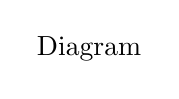
\begin{tikzpicture}
            \node {Diagram};
        \end{tikzpicture}
    \end{center}

